\begin{savequote}[75mm]
Passion is in all great searches and is necessary to all creative endeavors.
\qauthor{W. Eugene Smith}
\end{savequote}

\chapter{Search for Higgs pair production in boosted $\FourB$ final states}
\label{chap:boosted4b}

\section{Introduction}

After the discovery of the Higgs boson in the ATLAS Run 1 dataset and the subsequent measurements of its properties, the Higgs transformed into a potential tool in searches for physics beyond the Standard Model. The pair production cross section of the Higgs can be enhanced through BSM physics. Studying di-Higgs production also probes the Higgs self-coupling, shedding light on the structure of the Higgs potential. This chapter presents a search for resonant production of a Higgs pair in the $\FourBfull$ final state in $3.2 \ifb$ of data collected at $\sqrt{s} = 13 \TeV$. In particular, this chapter focuses on a search for this final state in the regime where $m_{X}$ is large ($\gtrsim 1 \TeV$) and the Higgs bosons in the decay are significantly boosted. A tailored selection for this boosted selection, using novel techniques in jet substructure and $b$-tagging, is discussed. Then, the data-driven background estimate is presented. Finally, the results of the search are shown. The signal models used as benchmarks are a spin-$2$ Rnadall Sundrum graviton (RSG) and a narrow width spin-$0$ resonance. These models are described in more detail in Chapter 1. Limits on signal models are reserved for the next chapter where the results of this chapter are combined with the results of a separate selection dedicated to the lower $m_X$ regime. 

\section{Motivation}

With the center of mass energy increase from $\sqrt{s} = 8 \TeV$ to $\sqrt{s} = 13 \TeV$, the LHC and ATLAS are able to probe new resonances at higher mass scales than previously accessible in Run 1. This is a powerful motivator for searching for a new resonance in the early $13 \TeV$ data. Figure~\ref{fig:lumi_ratio} shows the ratios of parton luminosities between $8$ and $13 \TeV$ for different resonance masses. For a resonance of $M_{X} = 2 \TeV$, the cross section at $\sqrt{s} = 13 \TeV$ is roughly a factor of $10$ larger than at $\sqrt{s} = 8 \TeV$. 

\begin{figure}[h!]
  %\vspace{20pt}
  \centering
  \captionsetup{justification=centering}

  %\hspace*{-32pt}
  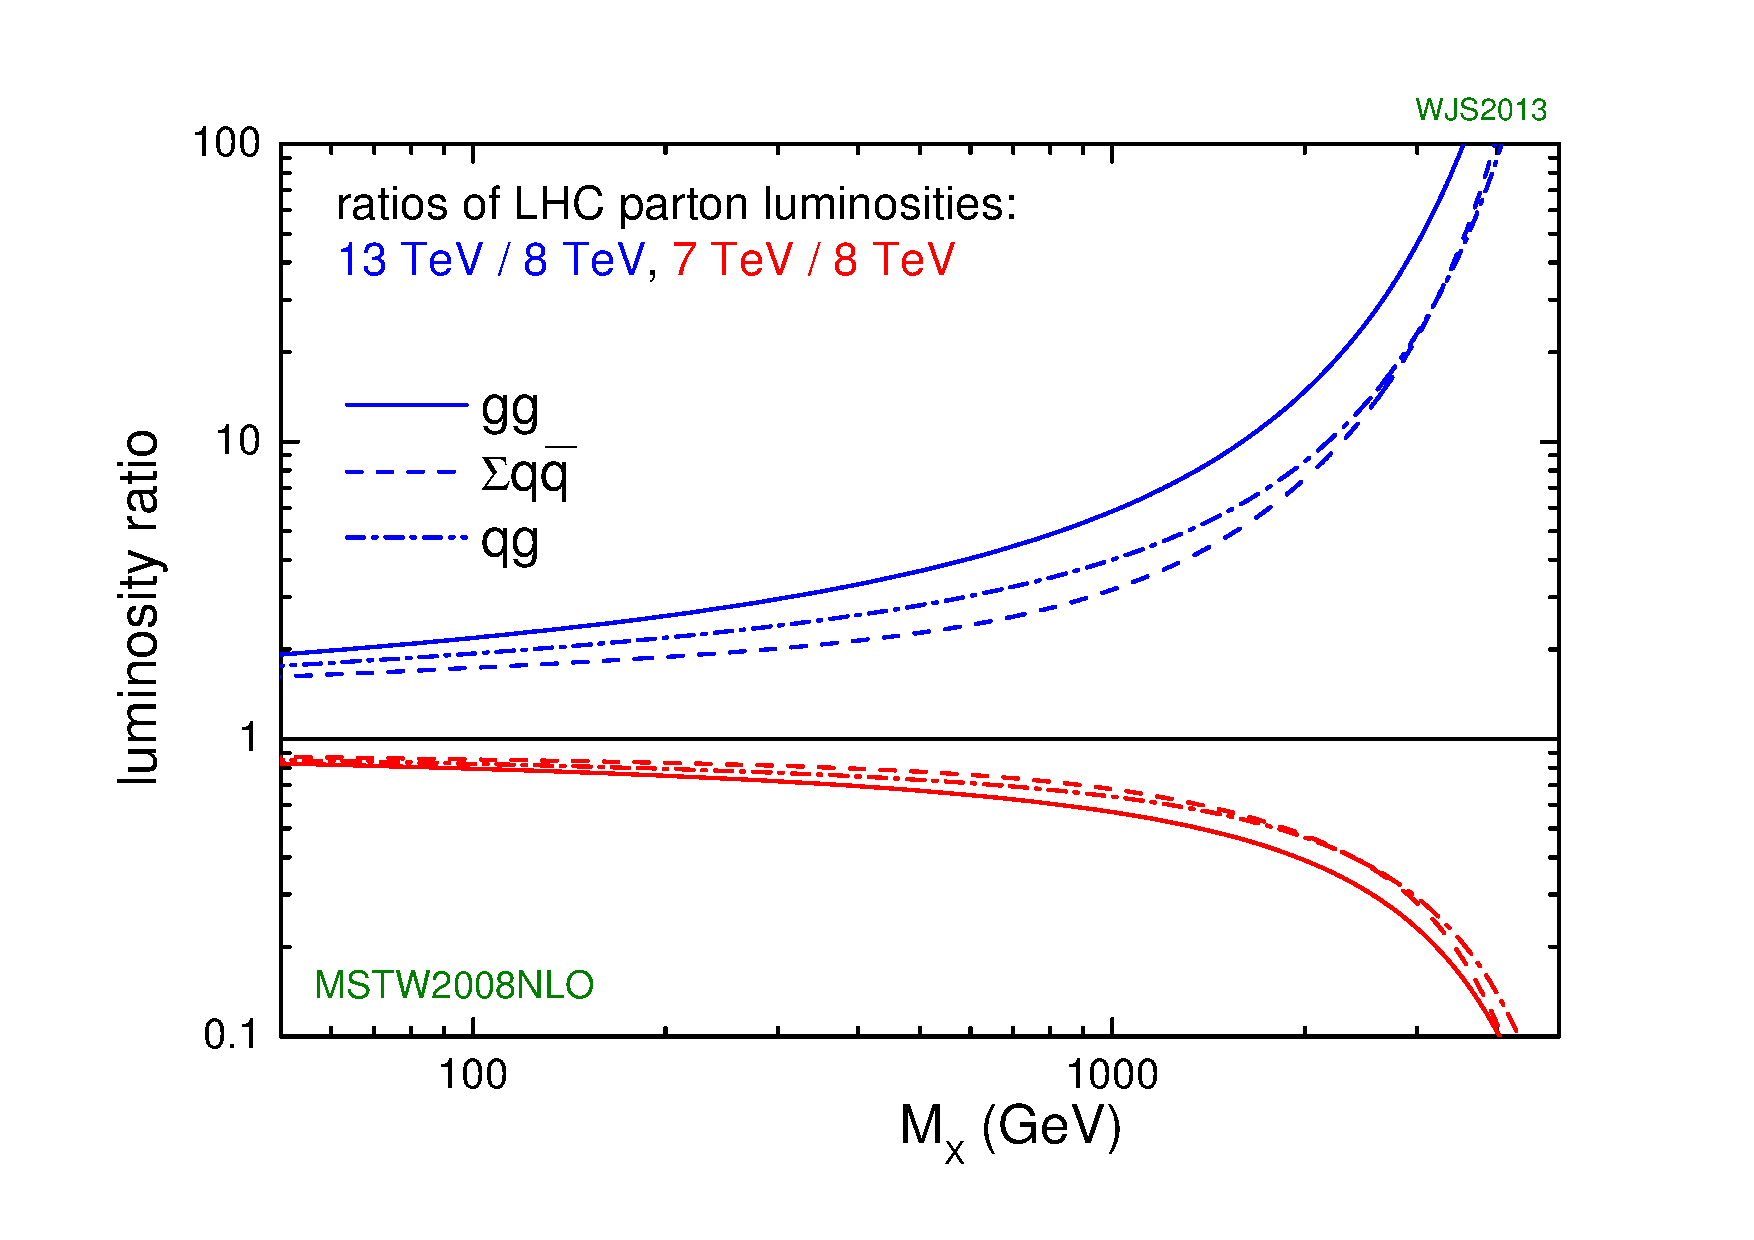
\includegraphics[width=0.6\textwidth,angle=270]{figures/Stirling_lumi_ratios}
  \caption{Parton luminosity ratios as a function of resonance mass $M_{X}$ for $13/8 \TeV$ and $7/8 \TeV$~\cite{LumiRatio}.}
  \label{fig:lumi_ratio}
\end{figure}

Higgs pair production offers a vast array of unprobed regions of phase space where searches for BSM physics can be made. Chapter 1 discusses some possibilities for both resonant and non-resonant enhancement of the di-Higgs production cross section. Given the increased mass reach of the LHC in Run 2, it is particularly important to focus on resonant searches at high $m_{X}$. One consideration when conducting a search in the $HH$ final state is which decay modes of the Higgs to consider. Figure~\ref{fig:HH_BR} shows the branching ratio of the $HH$ final state for different combinations of decays of each individual Higgs. As the largest branching ratio for the $125 \GeV$ Higgs is $H\to b\bar{b}$, the $HH\to b\bar{b}b\bar{b}$ branching ratio is also the largest at $33\%$. 

\begin{figure}[h!]
  %\vspace{20pt}
  \centering
  \captionsetup{justification=centering}

  %\hspace*{-32pt}
  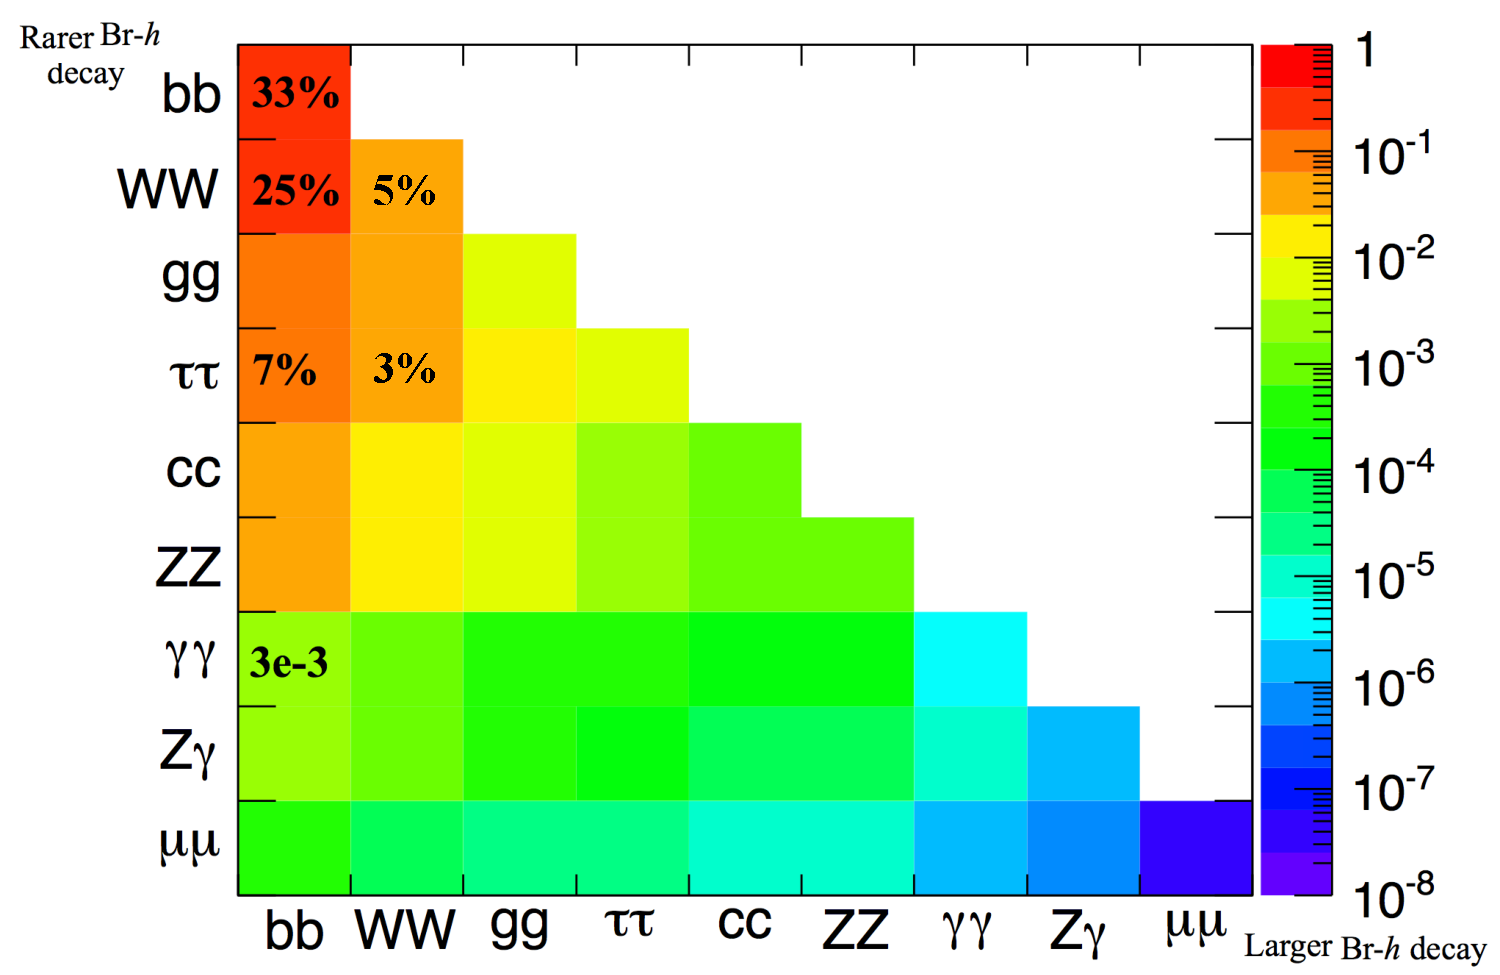
\includegraphics[width=0.8\textwidth]{figures/HH_BR}
  \caption{Summary of $HH$ branching ratios~\cite{HH_BR}.}
  \label{fig:HH_BR}
\end{figure}

At high $m_{X}$, the Higgs bosons resulting from the decay of a heavy resonance will have large $\pT$\footnote{In the limit that $m_{H} \ll m_{X}$, the Higgs $\pT$ is roughly $m_{X}/2$.}. The $\Delta R$ between the decay products of the Higgs is inversely proportional to the Higgs $\pT$, as shown in equation~\ref{eqn:bb_dr}. 

\begin{equation}
\Delta R \approx \frac{2m}{\pT}
\end{equation}

Figure~\ref{fig:bb_dr} shows the minimum $\Delta R$ between truth level $B$ decay vertices in simulation samples for Randall-Sundrum gravitons of different masses. The figure shows that as the mass of the graviton increases, the $\Delta R$ distribution between the $b$ quarks in the Higgs decay tends to shift to lower values. Because of this effect, it is necessary to tailor a selection to target these merged $b$-jets. 

\begin{figure}[h!]
  %\vspace{20pt}
  \centering
  \captionsetup{justification=centering}

  %\hspace*{-32pt}
  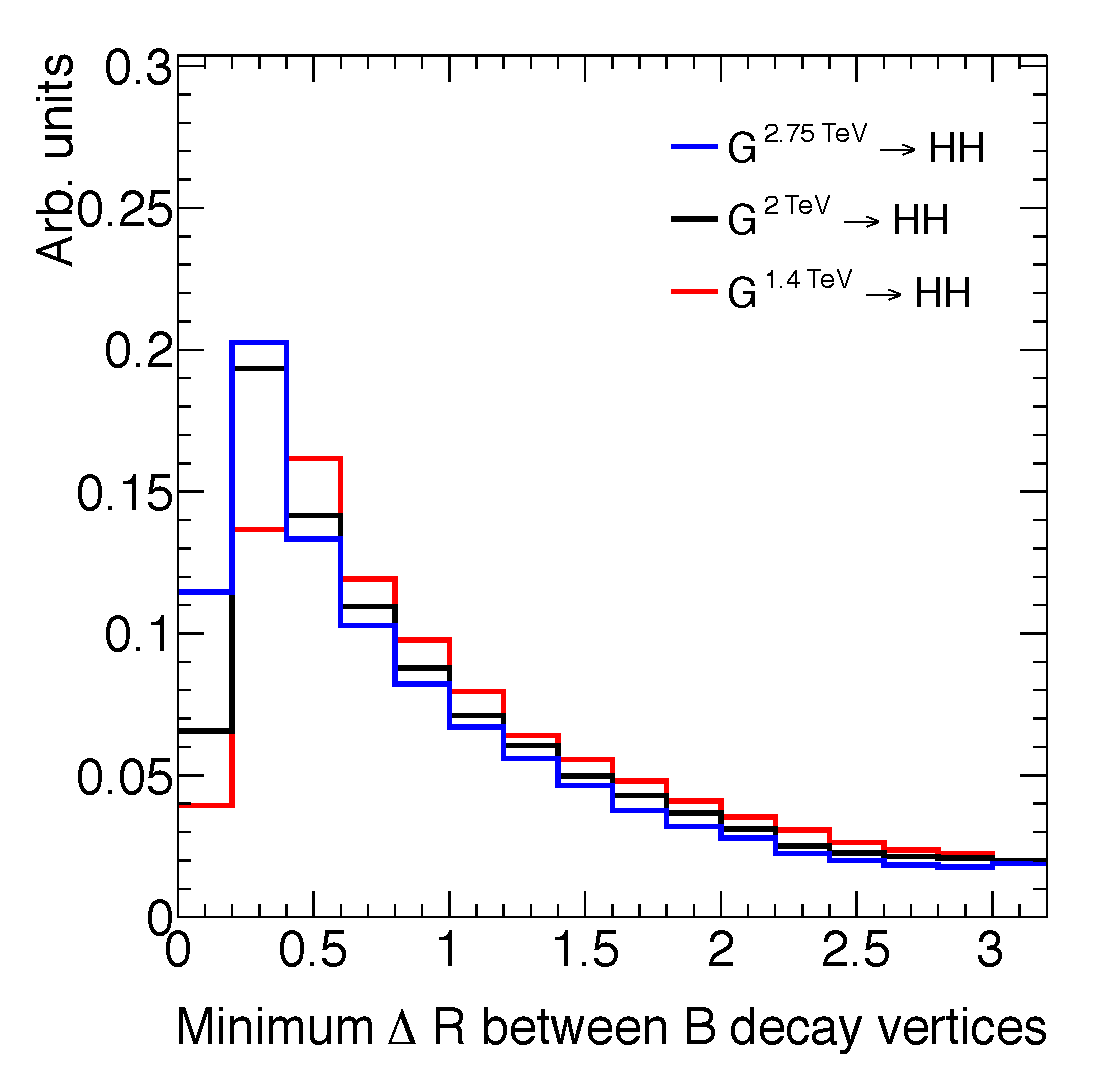
\includegraphics[width=0.5\textwidth]{figures/min_dR_bb}
  \caption{Minimum $\Delta R$ between $B$ decay vertices for different RSG masses in a $\Gkk \to HH \to 4b$ sample with $c = 1$}
  \label{fig:bb_dr}
\end{figure}

\section{Data and simulation samples}

\subsection{Signal models}

While the resonance search is by its nature generic (as it is a simple search for a peak in the $4b$ invariant mass spectrum), there are two signal models that the selection requirements have been optimized for. The first is  Randall-Sundrum (RSG) model, where a tower of massive spin-$2$ Kaluza-Klein gravitons is predicted. The second is a heavy narrow spin-$0$ resonance, the so-called ``heavy Higgs". This type of resonance arises, for example, in the two Higgs doublet model (2HDM). More details about the physics of these models and their motivation is given in chapter 1. 

Signal graviton ($\Gkk$) events are generated at leading order (LO) with \MADGRAPH 5 v$2.2.2$~\cite{MG5aMCatNLO}. The PDF set used is the \NNPDF 2.3 LO set~\cite{nnpdf}. For modeling parton shower and hadronization in jets, \PYTHIA $8.186$ is used with the A$14$ tune~\cite{pythia8,a14tune}. The free parameters in the RSG model are the graviton mass and the coupling constant $c \equiv k/\bar{M}_{\rm Pl}$\footnote{$k$ is the curvature constant for the warped extra dimension and $\bar{M}_{\rm Pl}$ is the Planck mass divided by $8\pi$}. Both the production cross section and width of the graviton are proportional to $c^2$. Samples are generated at both $c = 1$ and $c = 2$ for a variety of mass points between $300 \GeV$ and $3 \TeV$. 

The second signal sample is a heavy spin-$0$ resonance $H$ with a fixed width of $\Gamma_H = 1 \GeV$. This is generated with \MADGRAPH 5 and uses the \CT10 PDF set~\cite{ct10}. The parton shower and hadronization are handled by \HERWIG++ with the \CTEQ6L1 PDF set and the UEEE5 event tune~\cite{HerwigPP,cteq,UEEE5}. Because the width and branching ratios depend on 2HDM parameters, each mass point generated with this fixed width corresponds to a different point in the 2HDM parameter phase space. Mass points are generated between $300 \GeV$ and $1 \TeV$ as with the RSG signal samples. 

\subsection{Background samples}

While the dominant QCD multijet background is estimated with a fully data-driven method, the sub-dominant backgrounds $t\bar{t}$ and $Z$+jets are modeled with some input from simulation.

$\ttbar$ events are simulated at next-to-leading order (NLO) with the \POWHEGBOX version 1 generator using the \CT10 PDF set~\cite{PowhegBox}. The parton shower, hadronization, and underlying event are simulated with \PYTHIA 6.428 with the \CTEQ6L1 PDF set~\cite{pythia6}. The Perugia 2012 tune is used~\cite{Perugia2012}. NNLO QCD corrections to the cross sections are computed in Top++ 2.0~\cite{TopPP}. The top quark mass is set to $172.5 \GeV$. The shapes of distributions in $\ttbar$ are taken from MC while the normalization is taken from data.

Finally, the $Z$+jets background is simulated with \PYTHIA $8.186$ and the \NNPDF 2.3 LO PDF set. This background is negligible compared to the others and is taken fully from MC. 

\subsection{Data sample and trigger}

This analysis is done on $3.2 \ifb$ of data taken in $2015$ at $\sqrt{s} = 13 \TeV$. The details of the machine conditions during this time can be found in Chapter 2. Only data which was taken during stable beam conditions with all detectors functioning is used. Events must pass a trigger which requires a single $360 \GeV$ large radius ($R=1.0$) jet to be reconstructed in the HLT. Figure~\ref{fig:trig_eff_4b} shows the trigger efficiency for various trigger options as a function of graviton mass. Above $m_{G} > 1 \TeV$, the single large radius jet trigger is $99\%$ efficient for events passing the signal selection. 

\begin{figure}[h!]
  %\vspace{20pt}
  \centering
  \captionsetup{justification=centering}

  %\hspace*{-32pt}
  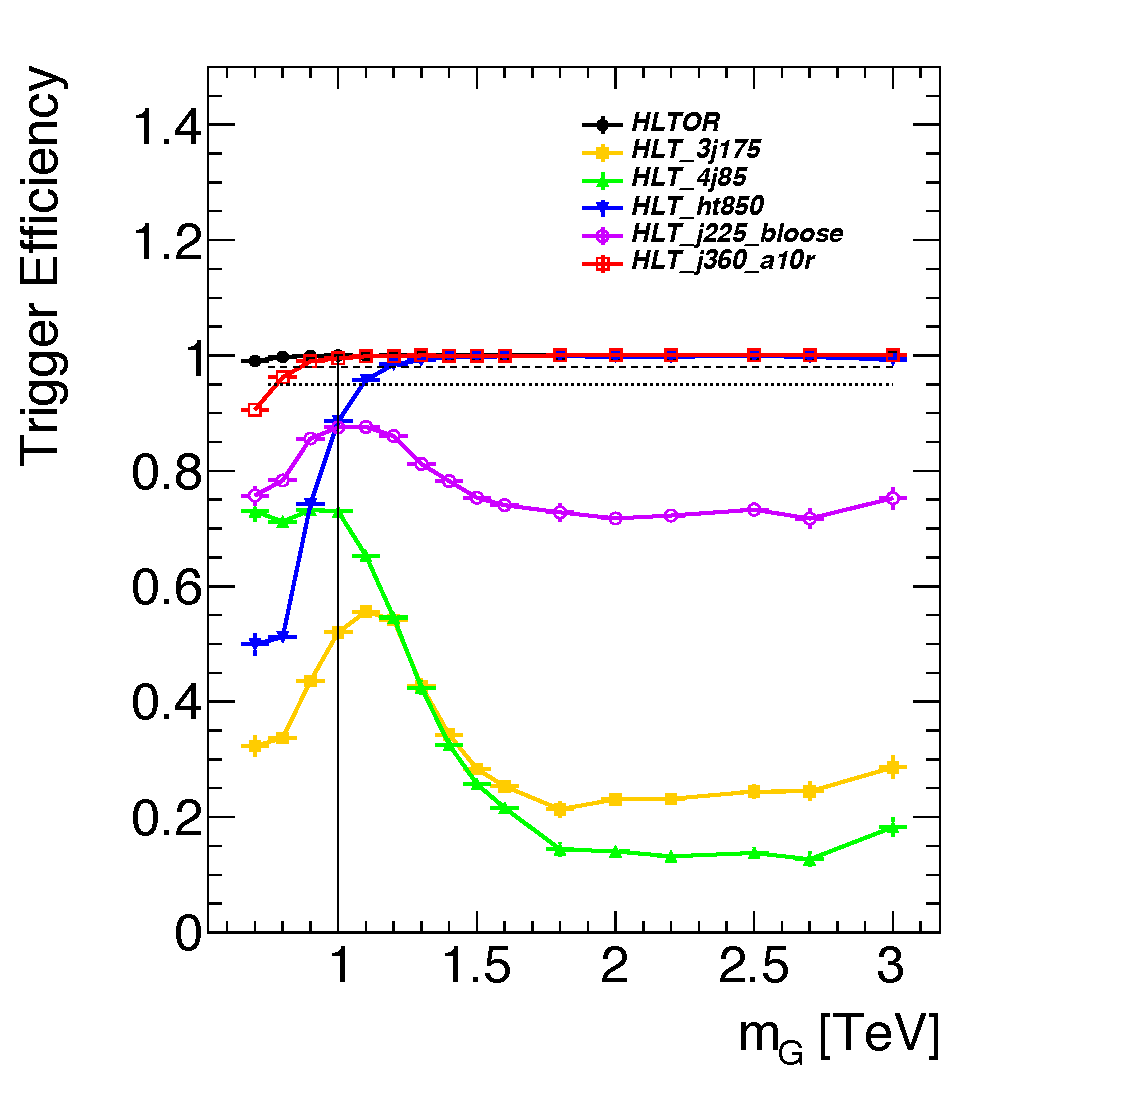
\includegraphics[width=0.7\textwidth]{figures/PassSignal_HLTeff}
  \caption{Trigger efficiency for events passing all signal region selections as a function of mass in $\Gkk \to HH \to 4b$ samples with $c = 1$~\cite{Tony}. In the trigger names, ``j" refers to a jet or jets. ``ht" refers to $H_{T}$, the scalar sum of transverse momenta in the event. ``bloose" refers to a loose $b$-tagging requirement applied to the jet. ``a10r" refers to anti-$k_{T}$ jets with $R = 1.0$. The numbers at the end are the thresholds on the given quantity in $\GeV$.}
  \label{fig:trig_eff_4b}
\end{figure}

\section{Event reconstruction}

The boosted selection first begins by defining a unique set of objects that can be exploited to increase signal efficiency in the kinematic regime where the final state $b$-jets are very merged. 

\subsection{Large radius ($R = 1.0$)\, jets}

The first step towards reconstructing the final state is to define objects that can be used to measure the kinematics of the Higgs bosons. In the boosted selection anti-$k_{T}$ jets with a radius parameter of $1.0$ are used. These jets is much larger in angular size than the typical $R=0.4$ jets and are intended to encompass both jets resulting from the Higgs decay\footnote{This is in contrast to the resolved selection, which uses two $R=0.4$ anti-$k_{T}$ jets for each Higgs}. The jets are built from clusters in the calorimeter calibrated with local calibration weighting~\cite{JetCalib}. 

Because of the large extent of these jets, great care must be taken to remove potential contrubutions of calorimeter clusters from pile-up. This is done using a technique called jet trimming~\cite{Trimming}. With trimming, the constituents of the large radius jet are re-clustered with a smaller radius with the $k_{T}$ algorithm. Then, these so-called subjets are removed from the larger jet if $p_{T}^{\rm subjet}/p_{T}^{\rm jet} < f_{\rm cut}$. In this analysis, the subjet radius is $R = 0.2$ and $f_{\rm cut} = 0.05$. Trimming has been shown to improve the mass resolution of large radius jets. Figure~\ref{fig:trimming} shows the effect of trimming on the large radius jet mass ($\MJ$). Because the large radius jet fully contains the higgs decay products, its invariant mass should correspond to the $125 \GeV$ mass of the Higgs. 

\begin{figure}[h!]
  %\vspace{20pt}
  \centering
  \captionsetup{justification=centering}

  %\hspace*{-32pt}
  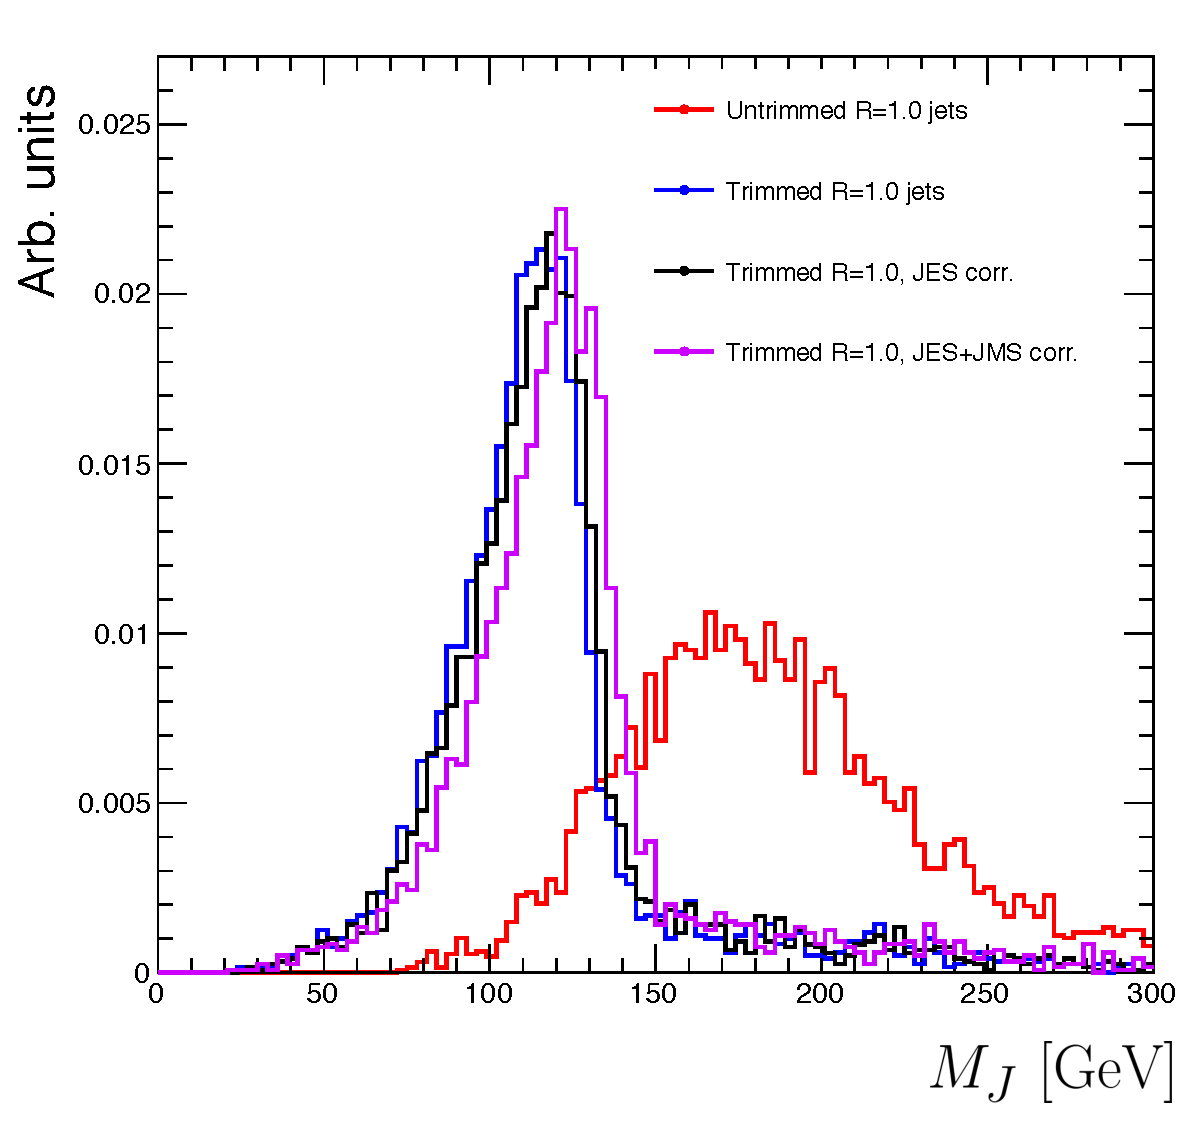
\includegraphics[width=0.6\textwidth]{figures/Trimmed_Mass}
  \caption{}
  \label{fig:trimming}
\end{figure}


\section{Event selection}

\section{Data-driven background estimation}

\section{Systematic uncertainties}

\section{Results}


